
\documentclass[12pt]{article}
\usepackage{graphicx}
\usepackage{float}
\usepackage{amsmath}
\usepackage{hyperref}
\usepackage{geometry}
\geometry{a4paper, margin=1in}

\title{Handwritten Digit Recognition on MNIST Dataset Using Convolutional Neural Networks}
\author{Mahla Entezari}
\date{Spring 2024}

\begin{document}

\maketitle

\begin{abstract}
Handwritten digit recognition has been a fundamental benchmark task in the field of machine learning and computer vision. This report investigates the performance of a simple Convolutional Neural Network (CNN) model on the MNIST dataset. We discuss the preprocessing techniques, model architecture, training procedures, experimental results, and insights obtained.
\end{abstract}

\section{Introduction}
The MNIST dataset of handwritten digits is one of the most studied datasets in the machine learning community. It serves as a standard benchmark for evaluating new techniques in image recognition. The goal of this project is to classify handwritten digits (0-9) from images using a Convolutional Neural Network.

\section{Related Work}
Numerous approaches have been proposed for handwritten digit recognition. Traditional methods involved feature engineering followed by classification algorithms. However, with the advent of deep learning, CNNs have significantly outperformed traditional methods by automatically learning hierarchical representations.

\section{Methodology}

\subsection{Dataset}
The MNIST dataset consists of 60,000 training images and 10,000 testing images. Each image is a grayscale, 28x28 pixels matrix.

\subsection{Preprocessing}
The images are normalized to have pixel values between 0 and 1. Labels are one-hot encoded to be compatible with categorical cross-entropy loss.

\subsection{Model Architecture}
The CNN model includes the following layers:
\begin{itemize}
    \item Convolutional layer with 32 filters, kernel size 3x3, activation ReLU
    \item MaxPooling layer with pool size 2x2
    \item Flatten layer
    \item Dense layer with 128 neurons, activation ReLU
    \item Output Dense layer with 10 neurons, activation softmax
\end{itemize}

\subsection{Training Details}
The model is trained using the Adam optimizer, with a categorical cross-entropy loss function. Training is performed for 5 epochs with a batch size of 128.

\section{Experiments}
The model is evaluated on both training and validation datasets during each epoch. Accuracy and loss metrics are recorded to monitor the training process.

\section{Results}

\subsection{Sample MNIST Images}
\begin{figure}[H]
    \centering
    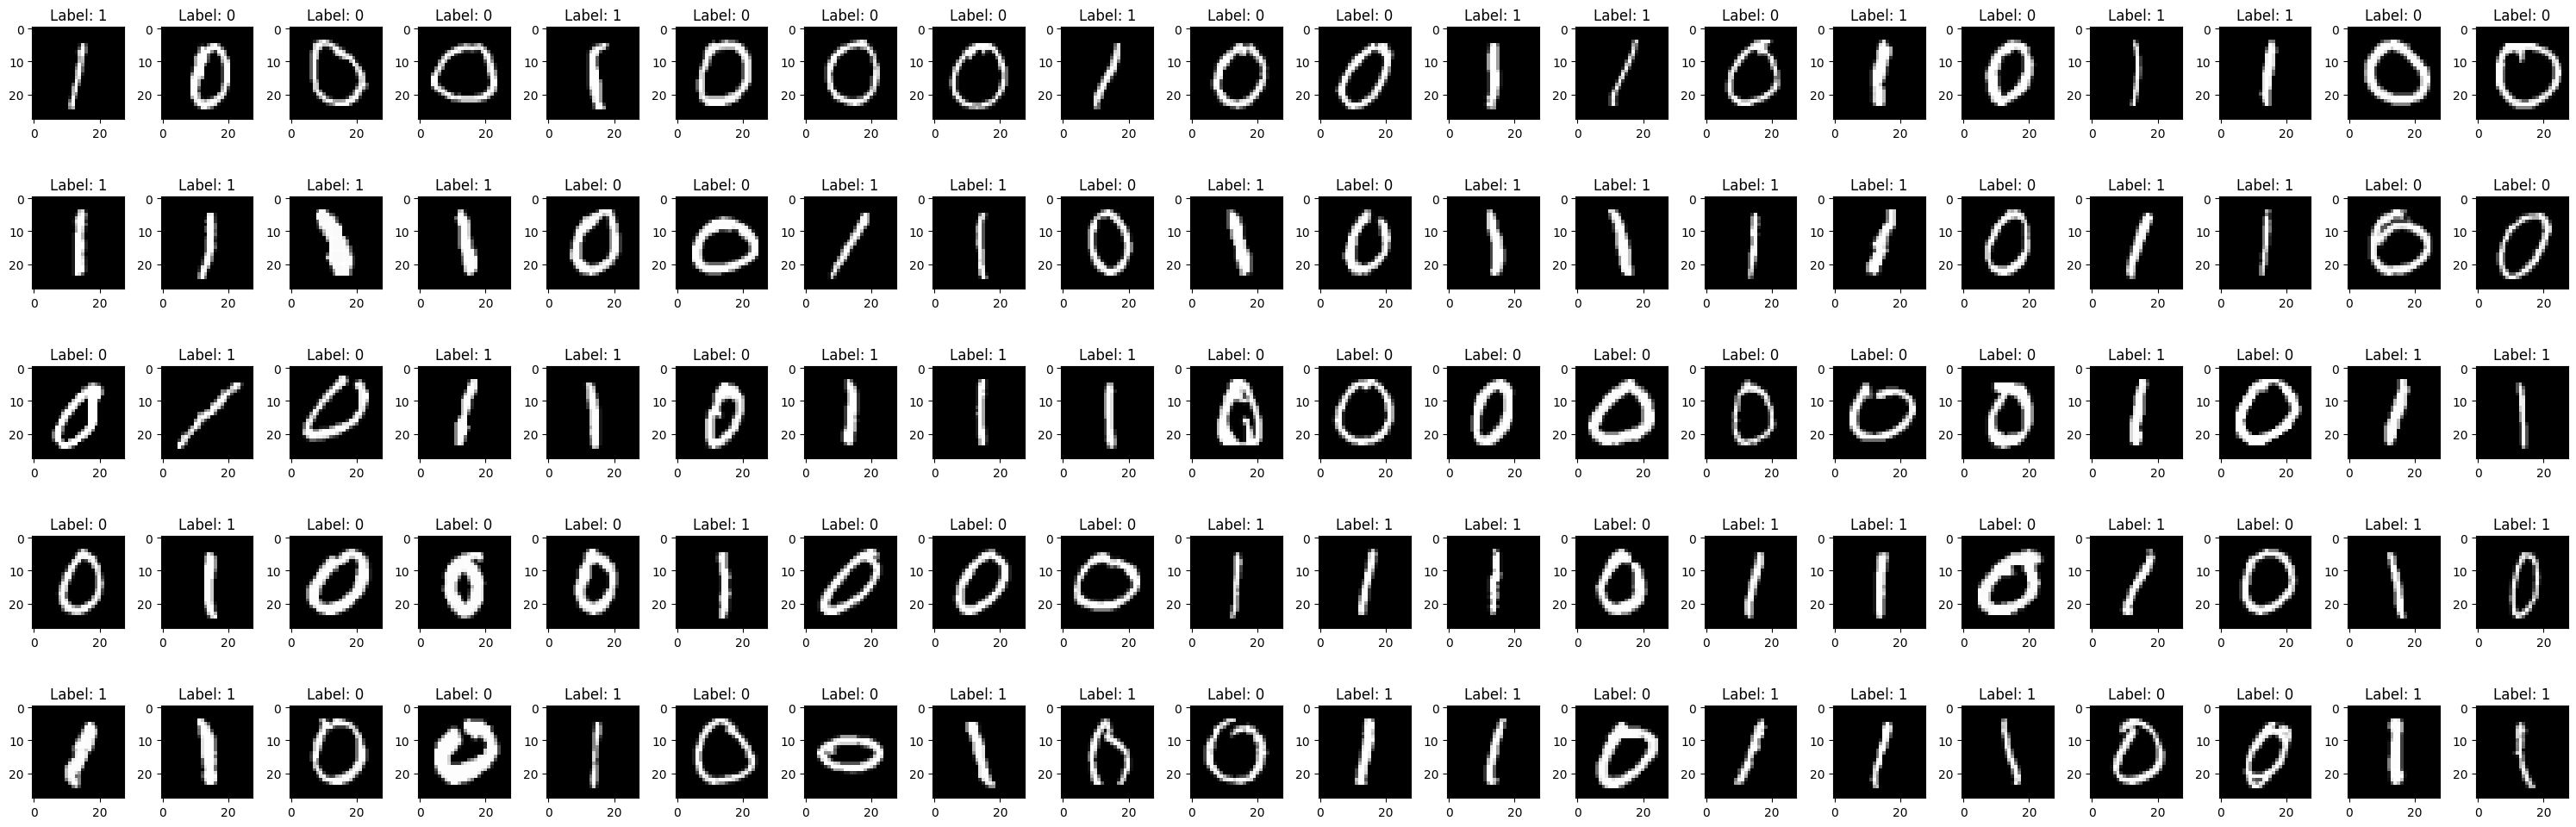
\includegraphics[width=\textwidth]{output2.png}
    \caption{Sample MNIST digits with labels}
\end{figure}

\subsection{Training and Validation Loss}
\begin{figure}[H]
    \centering
    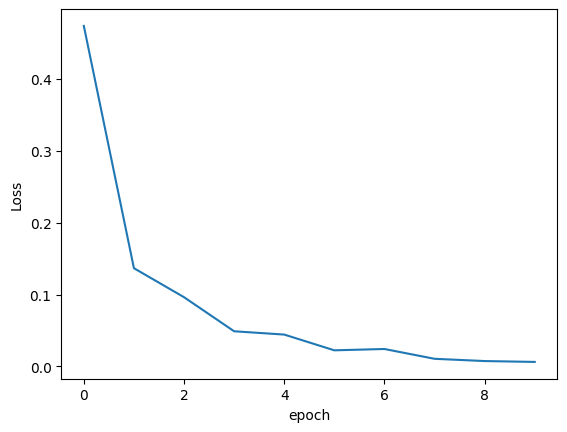
\includegraphics[width=0.8\textwidth]{output.png}
    \caption{Training Loss over Epochs}
\end{figure}

\section{Conclusion}
In this work, a basic CNN model was successfully applied to the MNIST handwritten digit recognition task. Even with a simple architecture, high accuracy was achieved, demonstrating the power of deep learning approaches for image classification problems. Future work can involve experimenting with deeper architectures or applying regularization techniques.

\section{References}
\begin{itemize}
    \item LeCun, Y., Bottou, L., Bengio, Y., \& Haffner, P. (1998). Gradient-based learning applied to document recognition. Proceedings of the IEEE.
    \item MNIST Database: \url{http://yann.lecun.com/exdb/mnist/}
\end{itemize}

\end{document}
